\documentclass[tikz,border=4pt]{standalone}
\usetikzlibrary{positioning, arrows.meta}

\tikzset{
  block/.style  = {draw, thick, fill=blue!6, minimum width=22mm, minimum height=11mm, align=center},
  sum/.style    = {draw, thick, circle, minimum size=6mm, inner sep=0pt},
  branch/.style = {circle, fill, inner sep=1.2pt},
  signal/.style = {inner sep=1pt},
  >={Stealth[length=2.5mm]},
}

\begin{document}
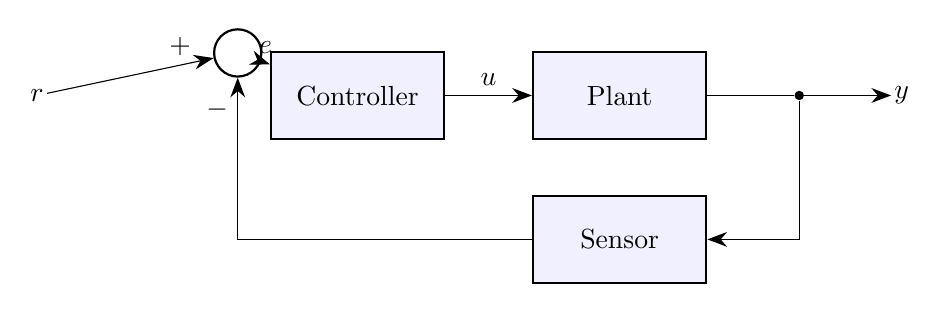
\begin{tikzpicture}[node distance=7mm and 11mm]
  \node[signal]                    (ref)    {$r$};
  \node[sum, above right=2mm and 2.2cm of ref]         (sum)    {};
  \node[block, right=2.83cm of ref]       (ctrl)   {Controller};
  \node[block, right=of ctrl]      (plant)  {Plant};
  \node[branch, right=of plant]    (split)  {};
  \node[signal, right=of split]    (out)    {$y$};
  \node[block, below=of plant]     (sensor) {Sensor};

  \draw[->] (ref)    -- node[pos=0.8, above] {$+$} (sum);
  \draw[->] (sum)    -- node[above] {$e$} (ctrl);
  \draw[->] (ctrl)   -- node[above] {$u$} (plant);
  \draw     (plant)  -- (split);
  \draw[->] (split)  -- (out);
  % The feedback path: down from the output, back under the loop, up into the sum.
  \draw[->] (split)  |- (sensor);
  \draw[->] (sensor) -| node[pos=0.9, left] {$-$} (sum);
\end{tikzpicture}
\end{document}
